%
% ---------------------------------------------------------------
% Copyright (C) 2012-2018 Gang Li
% ---------------------------------------------------------------
%
% This work is the default powerdot-tuliplab style test file and may be
% distributed and/or modified under the conditions of the LaTeX Project Public
% License, either version 1.3 of this license or (at your option) any later
% version. The latest version of this license is in
% http://www.latex-project.org/lppl.txt and version 1.3 or later is part of all
% distributions of LaTeX version 2003/12/01 or later.
%
% This work has the LPPL maintenance status "maintained".
%
% This Current Maintainer of this work is Gang Li.
%
%latex slides.tex 
%dvips slides.dvi
%ps2pdf slides.ps
\documentclass[
 size=14pt,
 paper=smartboard,  %a4paper, smartboard, screen
 mode=present, 		%present, handout, print
 display=slides, 	% slidesnotes, notes, slides
 style=tuliplab,  	% TULIP Lab style
 pauseslide,
 fleqn,leqno]{powerdot}

\usepackage{cancel}
\usepackage{caption}
\usepackage{stackengine}
\usepackage{smartdiagram}
\usepackage{attrib}
\usepackage{amssymb}
\usepackage{amsmath} 
\usepackage{amsthm} 
\usepackage{mathtools}
\usepackage{rotating}
\usepackage{graphicx}
\usepackage{boxedminipage}
\usepackage{rotate}
\usepackage{calc}
\usepackage[absolute]{textpos}
\usepackage{psfrag,overpic}
\usepackage{fouriernc}
\usepackage{pstricks,pst-3d,pst-grad,pstricks-add,pst-text,pst-node,pst-tree}
\usepackage{moreverb,epsfig,subfigure}
\usepackage{color}
\usepackage{booktabs}
\usepackage{etex}
\usepackage{breqn}
\usepackage{multirow}
\usepackage{natbib}
\usepackage{bibentry}
\usepackage{gitinfo2}
\usepackage{siunitx}
\usepackage{nicefrac}
\usepackage{media9}
\usepackage{animate}
\usepackage{auto-pst-pdf}
\usepackage{breakurl}
\usepackage{fontawesome}
\usepackage{xcolor}
\usepackage{multicol}



\usepackage{verbatim}
\usepackage[utf8]{inputenc}
\usepackage{dtk-logos}
\usepackage{tikz}
\usepackage{adigraph}
\usepackage{hyperref}
\usepackage{pgfplots}
\usepackage{verbatim}
\usepackage{fontawesome}


\usepackage{todonotes}
\usepackage{animate}
\usepackage{fontawesome}

\usepackage{listings}
\lstset{frameround=fttt,
frame=trBL,
stringstyle=\ttfamily,
backgroundcolor=\color{yellow!20},
basicstyle=\footnotesize\ttfamily}
\lstnewenvironment{code}{
\lstset{frame=single,escapeinside=`',
backgroundcolor=\color{yellow!20},
basicstyle=\footnotesize\ttfamily}
}{}


\usepackage{hyperref}
\hypersetup{ % TODO: PDF meta Data
  pdftitle={Presentation Title},
  pdfauthor={Gang Li},
  pdfpagemode={FullScreen},
  pdfborder={0 0 0}
}


% \usepackage{auto-pst-pdf}
% package to show source code

\definecolor{LightGray}{rgb}{0.9,0.9,0.9}
\newlength{\pixel}\setlength\pixel{0.000714285714\slidewidth}
\setlength{\TPHorizModule}{\slidewidth}
\setlength{\TPVertModule}{\slideheight}
\newcommand\highlight[1]{\fbox{#1}}
\newcommand\icite[1]{{\footnotesize [#1]}}

\newcommand\twotonebox[2]{\fcolorbox{pdcolor2}{pdcolor2}
{#1\vphantom{#2}}\fcolorbox{pdcolor2}{white}{#2\vphantom{#1}}}
\newcommand\twotoneboxo[2]{\fcolorbox{pdcolor2}{pdcolor2}
{#1}\fcolorbox{pdcolor2}{white}{#2}}
\newcommand\vpspace[1]{\vphantom{\vspace{#1}}}
\newcommand\hpspace[1]{\hphantom{\hspace{#1}}}
\newcommand\COMMENT[1]{}

\newcommand\placepos[3]{\hbox to\z@{\kern#1
        \raisebox{-#2}[\z@][\z@]{#3}\hss}\ignorespaces}

\renewcommand{\baselinestretch}{1.2}


\newcommand{\draftnote}[3]{
	\todo[author=#2,color=#1!30,size=\footnotesize]{\textsf{#3}}	}
% TODO: add yourself here:
%
\newcommand{\gangli}[1]{\draftnote{blue}{GLi:}{#1}}
\newcommand{\shaoni}[1]{\draftnote{green}{sn:}{#1}}
\newcommand{\gliMarker}
	{\todo[author=GLi,size=\tiny,inline,color=blue!40]
	{Gang Li has worked up to here.}}
\newcommand{\snMarker}
	{\todo[author=Sn,size=\tiny,inline,color=green!40]
	{Shaoni has worked up to here.}}

%%%%%%%%%%%%%%%%%%%%%%%%%%%%%%%%%%%%%%%%%%%%%%%%%%%%%%%%%%%%%%%%%%%%%%%%
% title
% TODO: Customize to your Own Title, Name, Address
%
\title{Jigsaw-Unintended-Bias-in-Toxicity-Classification-solution}
\author{
Pengcheng Jiang
\\
\\JiLin University
}
\date{\gitCommitterDate}


% Customize the setting of slides
\pdsetup{
% TODO: Customize the left footer, and right footer
rf=\href{http://www.tulip.org.au}{
Last Changed by: \textsc{\gitCommitterName}\ \gitVtagn-\gitAbbrevHash\ (\gitAuthorDate)
},
cf={Predict future sales},
}


\begin{document}

\maketitle

\begin{slide}[toc=,bm=]{Overview}
\tableofcontents[content=currentsection,type=1]
\end{slide}

\section{Problem Definition}

%%==========================================================================================
%%
\begin{slide}[toc=,bm=]{Jigsaw-Unintended-Bias-in-Toxicity-Classification-solution}
  \begin{center}
    \twotonebox{\parbox{.1\textwidth}{given}}{\parbox{.76\textwidth}
    {
      A tagged dataset containing comments
    }}
    \twotonebox{\parbox{.1\textwidth}{target}}{\parbox{.76\textwidth}
    {
      detect toxic comments and minimize unintended model bias.
    }}
    \twotonebox{\parbox{.1\textwidth}{evaluate}}{\parbox{.76\textwidth}
    {
      ACC
    }}
  \end{center}
\end{slide}
%%
%%==========================================================================================

\begin{slide}[toc=,bm=]{Train}
  \begin{center}
    \twotonebox{\parbox{.1\textwidth}{Data}}{\parbox{.76\textwidth}
    {
      \begin{figure}
        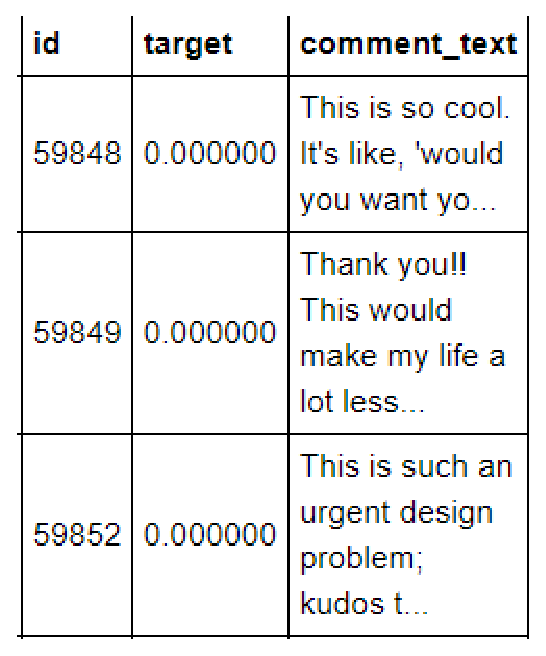
\includegraphics[scale=0.5]{picture/data.eps}
      \end{figure}
    }}
  \end{center}
\end{slide}


\section{Text preprocessing}


%%==========================================================================================
%%
\begin{slide}[toc=,bm=]{Text preprocessing}
  \begin{itemize}
    \item Count the total number of words contained in all texts, the maximum and minimum number of words contained in a text
    \item Check for missing data
    \item Change abbreviations to full:isn't -> is not(via dictionnary)
    \item clean_numbers
    \item Find all non alphabetic characters and clean_special_chars
    \item Solve the problem of misspelling words
    \item lower
  \end{itemize}
\end{slide}
%%
%%==========================================================================================


%%==========================================================================================
%%
\begin{slide}[toc=,bm=]{Text preprocessing}
        \begin{figure}
          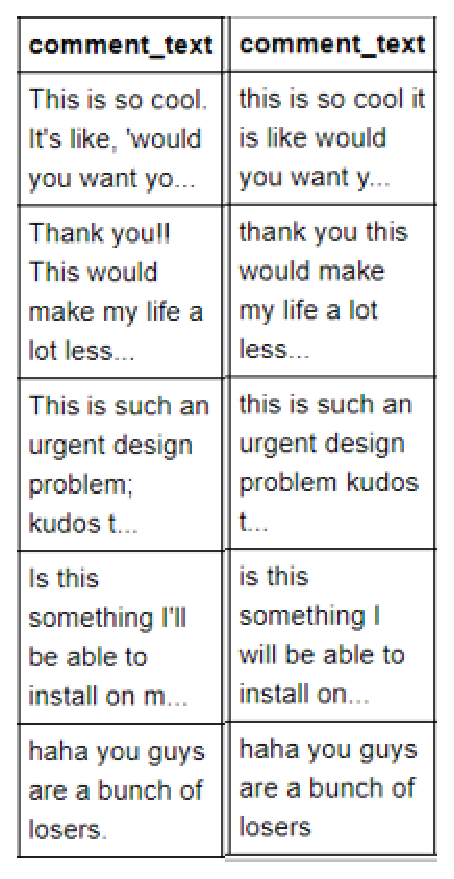
\includegraphics[scale=0.5]{picture/result.eps}
        \end{figure}  
\end{slide}
%%==========================================================================================
%%

\section{Embedding}
%%==========================================================================================
%%
\begin{slide}[toc=,bm=]{Tokenizer}
  \begin{center}
    \twotonebox{\parbox{.1\textwidth}{concept}}{\parbox{.76\textwidth}
    {
      What tokenizer does is actually very simple. It divides the words it sees into spaces, and then uses numbers to correspond one by one. Then we take the first num_ Words is the word with the highest frequency, others are not recognized.
    }}
    \twotonebox{\parbox{.1\textwidth}{Instruction}}{\parbox{.76\textwidth}
    {
      First learn the dictionary of the text, and then get the corresponding relationship between words and numbers, and then convert the text into a number string through this relationship, and then use the padding method to make up the number string to the same degree, then you can proceed to the next step : embedding
    }}
  \end{center}
\end{slide}
%%
%%==========================================================================================


%%==========================================================================================
%%
\begin{slide}[toc=,bm=]{Embedding}
  \begin{center}
      \twotonebox{\parbox{.1\textwidth}{Instruction}}{\parbox{.76\textwidth}
      {
        The embedding layer is the same as word2vec. Whether it is skip gram or cbow model, they infer each other from the context and the current, so we consider the relationship between the preceding and the following.
      }}
  \end{center}
\end{slide}
%%
%%==========================================================================================

\section{moudle}
%%==========================================================================================
%%
\begin{slide}[toc=,bm=]{LSTM}
  \begin{center}
      \twotonebox{\parbox{.1\textwidth}{Instruction}}{\parbox{.76\textwidth}
      {
        The embedding layer is the same as word2vec. Whether it is skip gram or cbow model, they infer each other from the context and the current, so we consider the relationship between the preceding and the following.
      }}

      \twotonebox{\parbox{.1\textwidth}{output}}{\parbox{.76\textwidth}
      {
        The embedding layer is the same as word2vec. Whether it is skip gram or cbow model, they infer each other from the context and the current, so we consider the relationship between the preceding and the following.
      }}
      \twotonebox{\parbox{.1\textwidth}{Dense}}{\parbox{.76\textwidth}
      {
        Map the result of LSTM to 0-1,activation='sigmoid'
      }}
  \end{center}
\end{slide}
%%
%%==========================================================================================


%%==========================================================================================
%%
\begin{slide}[toc=,bm=]{LSTM}
  \begin{center}
    \begin{figure}
      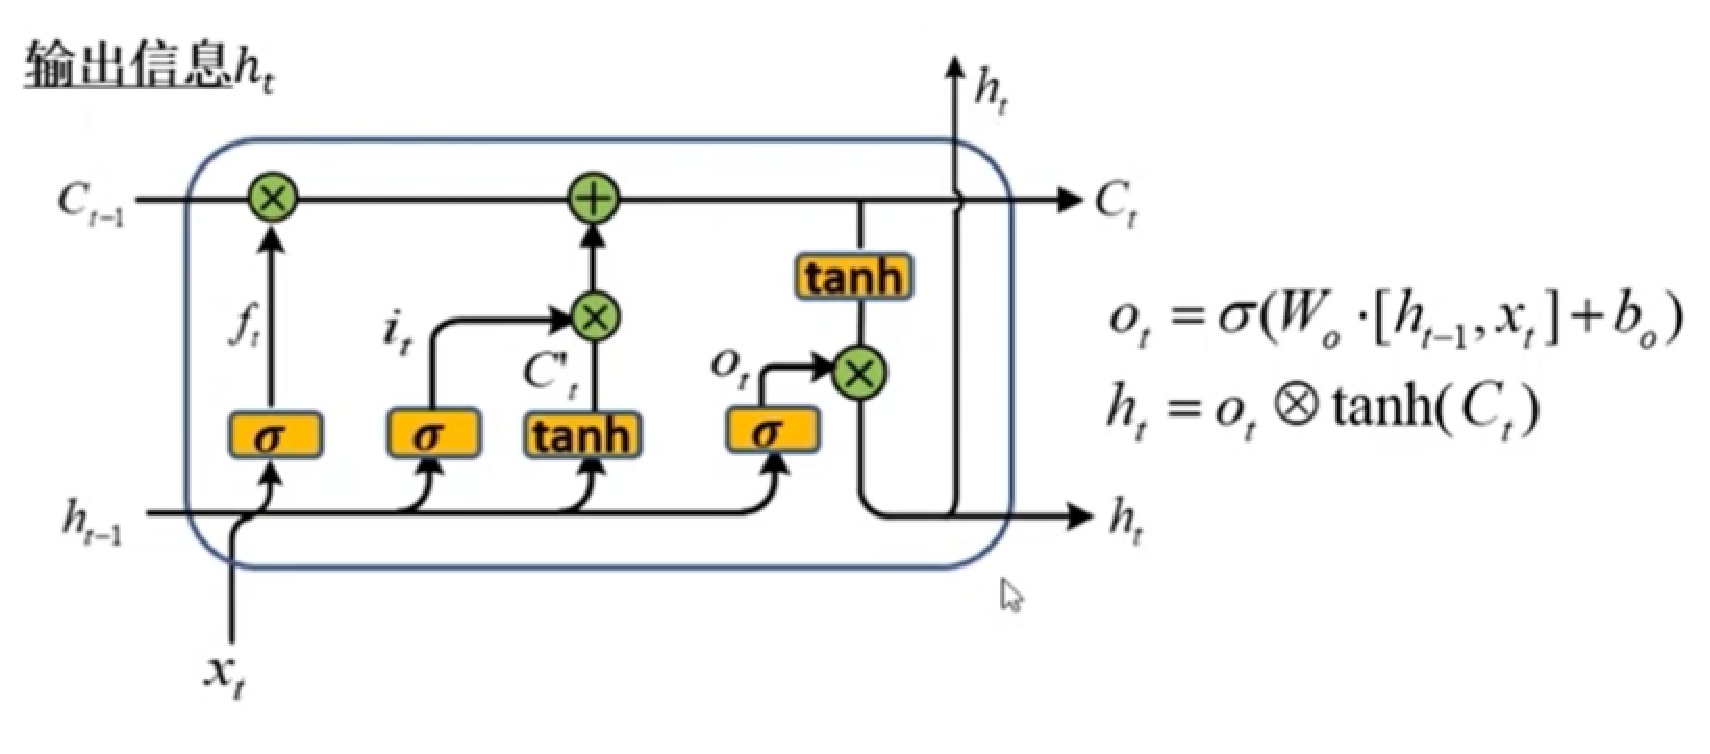
\includegraphics[scale=0.5]{picture/lstm.eps}
    \end{figure}
  \end{center}
\end{slide}
%%
%%==========================================================================================

%%==========================================================================================
%%
\begin{slide}[toc=,bm=]{Result}
  \begin{center}
    loss: 0.1937 - acc: 0.9401
  \end{center}
\end{slide}
%%
%%==========================================================================================


\end{document}
